\documentclass[11pt]{article}
\usepackage[preprint]{acl}
\usepackage{times,booktabs}
\usepackage[T1]{fontenc}
\usepackage{microtype}
\usepackage{tikz}

\title{How Far Can Verity Trust a Detector?\\
       Fall Custom Document, Revision 0}
\author{Calvin Salsali, Raymond Tao, Jaden Moore, Richard Han \\
        Team 23, Verity --- McMaster University}
\newcommand{\repo}{https://github.com/richy1337/Verity}
\newcommand{\papers}{\repo/blob/main/pdfs}

\begin{document}
\maketitle

\begin{abstract}
Verity needs to decide when the evidence about a selected item is too weak to show a direction. We trained two CPU-friendly text classifiers on the English Human ChatGPT Comparison Corpus (HC3) and tested a validation-tuned abstention rule on withheld questions and an unseen source domain. The character model reached 0.991 macro-$F_1$ on the 81\% of same-domain test answers it assessed, but improved on the word baseline by only 0.007 and falsely flagged 5 of the 27 Wikipedia-source human answers it assessed. A small image pilot missed every acceptance gate. The results support keeping the inconclusive outcome and treating these models as offline references.
\end{abstract}

\section{Task}

Verity is a browser extension for checking a selected passage or static image. Its result is a set of evidence signals and a suggestion for checking the source. This pilot asks a smaller question: can a light classifier distinguish a human answer from a ChatGPT answer under a stated error budget? The labels describe the source of a benchmark answer. They say nothing about whether it is accurate or whether a particular person wrote it.

The \href{\papers/SRS/SRS.pdf}{Software Requirements Specification (SRS)} calls for at least 0.80 macro-$F_1$, 70\% coverage, a false-positive rate (FPR) no greater than 10\%, and at least a 0.10 macro-$F_1$ gain over a declared baseline on the same assessed examples. These are engineering decision gates. Passing a gate on one corpus does not demonstrate safe use across the web. The \href{\papers/Design/SoftArchitecture/MG.pdf}{Module Guide} assigns extraction to M7/M8, assessment to M9 and offline evaluation to M10.

Our \href{\papers/DevelopmentPlan/DevelopmentPlan.pdf}{Development Plan} identifies pretrained neural detectors (\texttt{RoBERTa}/\texttt{DeBERTa} for text and \texttt{ViT}/\texttt{CLIP} with \texttt{EXIF}/\texttt{C2PA} metadata and Error Level Analysis for images) as full proof-of-concept candidates. For this Revision~0 Fall report, we intentionally execute CPU-only sparse TF--IDF and low-level RGB/gradient/frequency baselines first. Running fast deterministic pipelines verifies leak-free splitting, duplicate screening, sigmoid calibration, abstention tuning, and failure-to-decision gating before committing GPU compute or heavyweight inference dependencies.

\section{Related work}

\citet{guo2023hc3} collected paired human and ChatGPT answers and compared text detectors. Pairing on the prompt makes HC3 useful for an initial comparison. It still offers a narrow view of writing and one generation setting. \citet{dugan2024raid} show that detectors can degrade across new domains, generators, decoding choices and edits. Their RAID benchmark motivates a held-source check here and a later cross-generator test. DetectGPT uses probability curvature from a language model \citep{mitchell2023detectgpt}. A sparse classifier offers a CPU baseline that requires neither model access nor repeated generations. \citet{liang2023bias} show that false positives can concentrate on non-native English writing. We track false-positive counts and coverage by source. Source categories cannot establish a writer's first language.

For images, GenImage distinguishes in-generator and cross-generator evaluation \citep{zhu2023genimage}. CIFAKE is a useful small-image research comparison \citep{bird2024cifake}. Its native $32\times32$ images fall below Verity's $64\times64$ minimum. Neither synthetic-origin task covers the full range of digital edits that a browser user might ask about.

\section{Dataset and split}

HC3 English provides supervised labels from two answer fields. For each selected normalized question, we keep one human and one ChatGPT answer. We apply Unicode NFKC normalization and collapse whitespace. We keep answers with 150--10,000 characters after normalization. The model sees answer text only. Question text, label and source are excluded from its inputs.

We pick up to 1,400 eligible questions per source using a stable hash with seed 23. Finance, open question answering, Reddit Explain Like I'm Five and Wikipedia computer science/artificial intelligence contribute to internal splits. Medicine stays held out from fitting, calibration and threshold selection. A normalized question belongs to one partition. Questions listed across source domains are excluded. Stable hash buckets yield an approximate 70/10/10/10 training, calibration, validation and test split in the internal sources.

We remove exact normalized answer matches globally. We also compare word-trigram sets across partitions at Jaccard similarity of at least 0.85 and remove both members of a match. When one answer in a pair is removed, we drop the other as well. The verifier checks membership through hashed question and answer IDs. This audit catches literal and very close overlaps. Paraphrases with different trigrams and common prompts across unrelated datasets remain possible.

\begin{table}[h]
\centering
\begin{tabular}{lr}
\toprule
Partition & Answers \\
\midrule
Train & 5,664 \\
Calibration & 832 \\
Validation & 840 \\
Same-source test & 834 \\
Held-source test (medicine) & 2,378 \\
\bottomrule
\end{tabular}
\caption{Each partition contains equally many human and ChatGPT answers. Source snapshot and split IDs are in the experiment artifacts.}
\label{tab:splits}
\end{table}

\section{Models and procedure}

The baseline is word unigram/bigram term frequency--inverse document frequency (TF--IDF) with logistic regression. The candidate uses character 3--5 grams with the same classifier. Character grams can retain punctuation and word fragments that word tokenization discards. Both use sublinear term frequency, a minimum document frequency of 3, and at most 60,000 features. We fit the vectorizers only on training answers. The classifiers use $L_2$ regularization ($C=1$), a maximum of 1,000 iterations and the LIBLINEAR solver in scikit-learn. Logistic regression minimizes regularized binary log loss. We fixed these hyperparameters prior to running the pilot: unit regularization ($C=1$) provides a balanced un-tuned $L_2$ prior without overfitting to a small validation fold; $\texttt{min\_df}=3$ drops singleton artifacts and typos; $\texttt{max\_features}=60{,}000$ keeps CPU vectorization well within an 8\,GB laptop memory ceiling; and 1,000 LIBLINEAR iterations ensure full convex convergence. No neural training or test-set tuning was performed.

A second logistic regression fits a sigmoid to the character model's scores on the calibration fold. On the separate validation fold we sweep margins from 0 to 0.49 in steps of 0.01 (providing 50 uniform steps to avoid overfitting threshold boundaries on 840 items). We maximize assessed macro-$F_1$ among settings meeting the coverage and assessed FPR limits, with coverage as the tie-breaker. We freeze the chosen margin of 0.43 before reading test outcomes. A score at or below 0.07 gives the lower direction, and a score at or above 0.93 gives the higher direction. Scores in between abstain. This score reflects a balanced source-labelled corpus. It should not be read as the probability that a passage on the web is synthetic.

The run used Python 3.12.15 and scikit-learn 1.8.0 on an ARM64 Mac with CPU execution. The two classifier fits together took about six seconds. The experiment records batch timing for reproducibility. Browser and network latency are separate product tests.

\section{Results}

Table~\ref{tab:results} compares models on identical assessed items. Coverage divides the number of assessed items by the eligible test count. Assessed FPR divides false flags by the number of assessed human items. FPR over all eligible human items is reported separately in the artifacts. When an answer abstains, the full-population diagnostic counts it as a miss for the true class. Forced classification is an additional diagnostic that applies a 0.5 threshold to every answer.

\begin{table}[h]
\centering
\small
\begin{tabular}{@{}lrr@{}}
\toprule
Metric & Same source & Medicine \\
\midrule
Assessed / eligible & 675/834 & 1,985/2,378 \\
Coverage & 80.9\% & 83.5\% \\
Assessed candidate $F_1$ & .991 & .999 \\
Word baseline $F_1$ & .984 & .996 \\
Gain over word baseline & .007 & .004 \\
Assessed false flags (FPR) & 5/322 & 0/801 \\
Forced candidate $F_1$ & .953 & .969 \\
Full-population $F_1$ & .886 & .901 \\
\bottomrule
\end{tabular}
\caption{Held-out text results. False flag counts are conditional on an assessed human answer.}
\label{tab:results}
\end{table}

The character model clears the aggregate $F_1$, coverage and FPR floors on both tests and misses the baseline-improvement gate on both. The prior-only baseline gives 0.333 macro-$F_1$ on balanced classes. Comparing only to it would hide how much an ordinary word model already explains. With abstentions disabled, the word model slightly leads the character model on medicine ($0.972$ versus $0.969$). The gain on the selected examples is small enough that this result gives no reason to commit the product to the character model.

\paragraph{Where it fails.}
Figure~\ref{fig:source-breakdown} disaggregates coverage and assessed FPR across all five test sources. All five same-source false flags occur in the Wikipedia-derived source, where 27 human answers received a direction and five of them were flagged (18.5\%). That source covered only 59.6\% of its 146 items, failing both the 70\% coverage floor and 10\% FPR ceiling simultaneously. Across medicine, the system assessed 67.4\% of human answers and 99.6\% of ChatGPT answers. Zero assessed false flags there should be read alongside that imbalance. Among medicine answers near the eligibility floor (150--299 characters), only one of 253 was ChatGPT-labelled and the model missed it. That slice is too imbalanced to support conclusions about short generated answers.

\begin{figure*}[t]
\centering
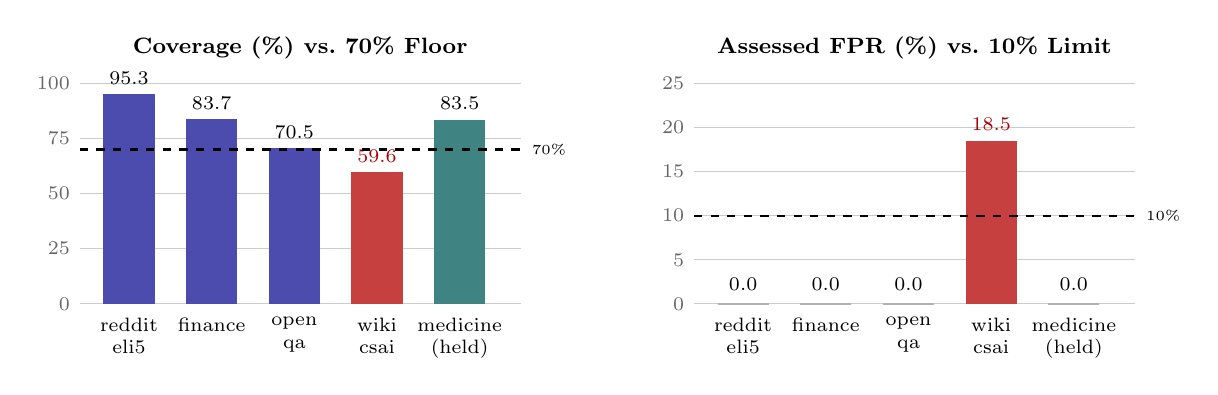
\begin{tikzpicture}[font=\scriptsize, x=1cm, y=1cm]
  % Left panel: Coverage (%) [0, 100] mapped to y in [0, 2.8] => scale 0.028/pct
  \node[font=\footnotesize\bfseries] at (2.8, 3.25) {Coverage (\%) vs.\ 70\% Floor};
  \draw[gray!40] (0, 0) -- (5.6, 0);
  \draw[gray!40] (0, 0.7) -- (5.6, 0.7);
  \draw[gray!40] (0, 1.4) -- (5.6, 1.4);
  \draw[gray!40] (0, 2.1) -- (5.6, 2.1);
  \draw[gray!40] (0, 2.8) -- (5.6, 2.8);
  \foreach \pct/\yy in {0/0, 25/0.7, 50/1.4, 75/2.1, 100/2.8} {
    \node[left, gray!80!black] at (0, \yy) {\pct};
  }
  % Bars: reddit_eli5=95.3, finance=83.7, open_qa=70.5, wiki_csai=59.6, medicine=83.5
  \fill[blue!55!black!70]   (0.30, 0) rectangle (0.95, 2.668); \node[above] at (0.625, 2.668) {95.3};
  \fill[blue!55!black!70]   (1.35, 0) rectangle (2.00, 2.344); \node[above] at (1.675, 2.344) {83.7};
  \fill[blue!55!black!70]   (2.40, 0) rectangle (3.05, 1.974); \node[above] at (2.725, 1.974) {70.5};
  \fill[red!70!black!75]    (3.45, 0) rectangle (4.10, 1.669); \node[above, red!65!black] at (3.775, 1.669) {59.6};
  \fill[teal!70!black!75]   (4.50, 0) rectangle (5.15, 2.338); \node[above] at (4.825, 2.338) {83.5};
  % MIN_COVERAGE dashed line at 70% => y=1.96
  \draw[dashed, thick, black] (0, 1.96) -- (5.6, 1.96);
  \node[right, font=\tiny] at (5.62, 1.96) {70\%};
  % X labels
  \node[below, align=center] at (0.625, -0.05) {reddit\\eli5};
  \node[below, align=center] at (1.675, -0.05) {finance};
  \node[below, align=center] at (2.725, -0.05) {open\\qa};
  \node[below, align=center] at (3.775, -0.05) {wiki\\csai};
  \node[below, align=center] at (4.825, -0.05) {medicine\\(held)};

  % Right panel: Assessed FPR (%) [0, 25] mapped to y in [0, 2.8] => scale 0.112/pct
  \begin{scope}[xshift=7.8cm]
    \node[font=\footnotesize\bfseries] at (2.8, 3.25) {Assessed FPR (\%) vs.\ 10\% Limit};
    \draw[gray!40] (0, 0) -- (5.6, 0);
    \draw[gray!40] (0, 0.56) -- (5.6, 0.56);
    \draw[gray!40] (0, 1.12) -- (5.6, 1.12);
    \draw[gray!40] (0, 1.68) -- (5.6, 1.68);
    \draw[gray!40] (0, 2.24) -- (5.6, 2.24);
    \draw[gray!40] (0, 2.80) -- (5.6, 2.80);
    \foreach \pct/\yy in {0/0, 5/0.56, 10/1.12, 15/1.68, 20/2.24, 25/2.80} {
      \node[left, gray!80!black] at (0, \yy) {\pct};
    }
    % Bars: reddit=0.0, finance=0.0, open_qa=0.0, wiki=18.5 (2.072), medicine=0.0
    \draw[gray!60, thick] (0.30, 0) -- (0.95, 0); \node[above] at (0.625, 0.04) {0.0};
    \draw[gray!60, thick] (1.35, 0) -- (2.00, 0); \node[above] at (1.675, 0.04) {0.0};
    \draw[gray!60, thick] (2.40, 0) -- (3.05, 0); \node[above] at (2.725, 0.04) {0.0};
    \fill[red!70!black!75] (3.45, 0) rectangle (4.10, 2.072); \node[above, red!65!black] at (3.775, 2.072) {18.5};
    \draw[gray!60, thick] (4.50, 0) -- (5.15, 0); \node[above] at (4.825, 0.04) {0.0};
    % MAX_FPR dashed line at 10% => y=1.12
    \draw[dashed, thick, black] (0, 1.12) -- (5.6, 1.12);
    \node[right, font=\tiny] at (5.62, 1.12) {10\%};
    % X labels
    \node[below, align=center] at (0.625, -0.05) {reddit\\eli5};
    \node[below, align=center] at (1.675, -0.05) {finance};
    \node[below, align=center] at (2.725, -0.05) {open\\qa};
    \node[below, align=center] at (3.775, -0.05) {wiki\\csai};
    \node[below, align=center] at (4.825, -0.05) {medicine\\(held)};
  \end{scope}
\end{tikzpicture}
\caption{Per-source coverage and assessed false-positive rate (FPR) for the character 3--5 gram text model at validation margin $0.43$. Only \texttt{wiki\_csai} fails both SRS gates simultaneously ($59.6\% < 70\%$ coverage; $5/27 = 18.5\% > 10\%$ FPR), while held-out \texttt{medicine} attains $0.0\%$ assessed FPR alongside asymmetric class coverage ($67.4\%$ human vs.\ $99.6\%$ ChatGPT).}
\label{fig:source-breakdown}
\end{figure*}

\paragraph{What calibration changed.}
On the same-source test, the Brier score fell from 0.060 to 0.036 after sigmoid calibration. It fell from 0.046 to 0.023 in medicine. Training forced macro-$F_1$ was 0.983, compared with 0.953 on the internal test, a 0.030 gap. These differences are consistent with some training fit and corpus-specific style effects. They cannot distinguish stable authorship signals from recurring formatting or boilerplate cues. Both test partitions still come from the same dataset and generation setup.

\section{Image pilot}

We sampled 192 labelled examples from Tiny-GenImage: 96 training, 32 validation, and 64 held-out test images, balanced between original photographs and generated images. We selected fixed windows in the published train and validation splits before fitting. The files served by the dataset viewer all met the product size and static-format bounds. A byte-hash check and a 64-bit difference-hash screen found no pair within the chosen cutoff. The mirror does not expose original photograph or prompt group IDs, so this is a smoke test. It cannot establish source separation or cross-generator robustness.

We converted each image to red, green and blue channels and resized to $64\times64$ for feature extraction. The baseline uses per-channel means and standard deviations. The candidate adds grayscale gradient statistics and frequency-band energy. Both use training-set standardization and $L_2$ logistic regression ($C=1$) in scikit-learn. We used model scores directly because the validation set was too small to set aside another calibration fold. No margin met both validation limits. The fallback margin of 0.09 minimized assessed FPR among margins that kept 70\% coverage on validation. It is for comparison only.

On the 64 held-out examples the candidate assessed 43 (67.2\%), attained 0.581 macro-$F_1$, and flagged 11 of 23 assessed authentic images (Table~\ref{tab:image-results}). The colour baseline scored 0.650 on the same items. Re-encoding those same inputs as JPEG at quality 60 kept the selective confusion counts unchanged. Forced macro-$F_1$ dropped from 0.547 to 0.531. These are paired observations, so the JPEG copies do not increase the number of independent test items. Because the model missed every gate (\texttt{MIN\_COVERAGE} $70.0\%$, \texttt{MIN\_F1\_SCORE} $0.80$, $+0.10$ baseline delta, and \texttt{MAX\_FPR} $10.0\%$), the Development Plan failure-to-decision rule triggers immediately: directional visual classification is blocked in Revision~0, and browser-facing image checks remain restricted to deterministic \texttt{EXIF}/\texttt{C2PA} metadata inspection (\texttt{FR13}) until pretrained \texttt{ViT}/\texttt{CLIP} candidates pass on an auditable cross-generator dataset.

\begin{table}[h]
\centering
\footnotesize
\setlength{\tabcolsep}{4pt}
\begin{tabular}{@{}lrr@{}}
\toprule
Metric & Clean test & JPEG-60 \\
\midrule
Assessed / eligible & 43/64 & 43/64 \\
Coverage & 67.2\% & 67.2\% \\
Assessed candidate $F_1$ & .581 & .581 \\
Colour baseline $F_1$ & .650 & .650 \\
Gain over baseline & $-$.069 & $-$.069 \\
Assessed false flags & 11/23 (47.8\%) & 11/23 (47.8\%) \\
Forced candidate $F_1$ & .547 & .531 \\
Full-population $F_1$ & .467 & .467 \\
\bottomrule
\end{tabular}
\caption{Held-out Tiny-GenImage pilot metrics ($n=64$) under clean serving and paired JPEG-60 re-encoding.}
\label{tab:image-results}
\end{table}

This pilot uses synthetic-origin labels. It did not measure editing or authenticity. Camera metadata and Content Credentials should remain separate observations, because ordinary re-encoding can remove them. The next image comparison needs auditable source groups, a held-out generator and more authentic compressed images.

\section{What changes in Verity}

We would keep the sparse models as offline references and leave directional classification gated behind stronger evidence. For the next comparison, the word model stays frozen as a reference while pretrained text and image candidates are tested on wholly separate sources. NFR1 needs the same eligibility rules and baseline subset for every model. NFR10 needs actual language-background and recompression slices, with their sample counts and abstentions. HC3 source names do not substitute for those labels.

The TA's feedback on acceptance criteria asks for an explanation of the targets and a clear decision when they are missed. The 0.10 gain is a provisional requirement for adopting extra model complexity. Under our Development Plan decision rules, missing that gate on HC3 means the character classifier stays offline-only while \texttt{RoBERTa}/\texttt{DeBERTa} candidates are evaluated on RAID plus explicit ESL/formal slices. On the image path, missing all four gates on Tiny-GenImage blocks directional classification in favour of descriptive \texttt{EXIF}/\texttt{C2PA} metadata until \texttt{ViT}/\texttt{CLIP} evaluation completes. A detector that clears aggregate gates but misses a source or subgroup FPR limit (as on \texttt{wiki\_csai}) needs investigation and an explicit scope decision before use. For the interface, M9 owns the decision about applicability and abstention. M3 displays the reason, states the limitation, and suggests a source check. An authentic item can still be flagged, so the model result belongs alongside the evidence and a plain-language false-positive warning.

\section{Data and reproducibility}

The experiment uses public benchmark data from the source maintainers. HC3's source-specific terms apply where stricter than its general CC BY-SA 4.0 terms. Tiny-GenImage is marked CC BY-NC-SA 4.0 by its mirror. We use that sample for academic evaluation. No dataset text, image payload or live user content is committed. Each prediction retains an item hash, label, score, split and outcome. Baseline comparisons and error counts can be reconstructed from those records. The \href{\repo/tree/main/docs/CDs/MLReport/experiment}{experiment directory} records the commands, checksums, outcome records and environment. A same-environment replay tests repeatability. Cross-member reproduction on another machine and the larger SRS acceptance evaluation remain open.

\section*{Contribution and AI disclosure}

Raymond Tao owns detection and benchmark design, audited \texttt{run\_text.py} and \texttt{run\_image.py}, independently recomputed every partition count, coverage proportion, assessed/forced/full-population macro-$F_1$, assessed FPR, and baseline delta directly from \texttt{text/\allowbreak{}predictions.json.gz} and \texttt{image/\allowbreak{}predictions.json.gz} against \texttt{metrics.json} (confirming agreement within $10^{-12}$), and verified Tables~1--3 and Figure~1 against the serialized experiment records. Calvin Salsali directed Revision~0 preparation, confirmed the approved Fall ML Model Report deliverable (\texttt{ExceptionsGranted.md}), and reviewed alignment with the M3 uncertainty banner and false-positive warning requirements. Jaden Moore reviewed alignment between the pilot pipeline boundaries (\texttt{M7}--\texttt{M10}) and the Development Plan decision gates, and Richard Han audited the split manifests, dataset SHA-256 checksums, zero-raw-payload retention in the \texttt{experiment/} artifacts, and final compiled PDF.

Generative AI assistance during script development, metric comparison, and \LaTeX{} drafting included \textbf{OpenAI Codex (GPT-6.1)}, \textbf{Anthropic Claude Sonnet 5.5}, \textbf{Google Gemini Flash 3.8}, and \textbf{Google Gemini 4 Hydrogen}. All reported numbers, citations, plots, and architectural claims were verified against repository artifacts by the named team members prior to submission.

\bibliography{custom}
\end{document}
